\documentclass[border=6pt]{standalone}
\usepackage{tikz}
\usetikzlibrary{arrows.meta,calc,positioning}
\begin{document}
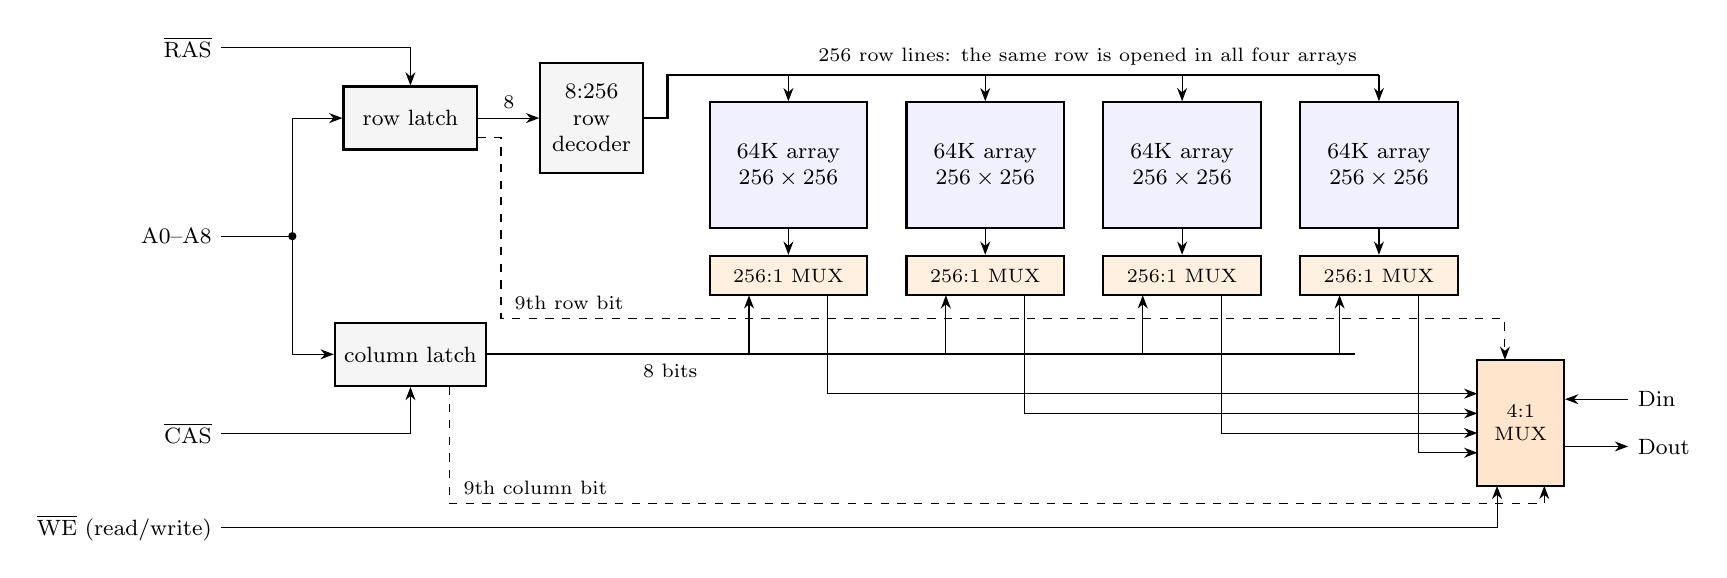
\begin{tikzpicture}[>=Stealth,font=\small,
 blk/.style={draw,thick,fill=gray!8,align=center,font=\footnotesize,minimum height=0.8cm},
 arr/.style={draw,thick,fill=blue!6,align=center,font=\footnotesize,minimum width=2.0cm,minimum height=1.6cm},
 mx/.style={draw,thick,fill=orange!12,align=center,font=\scriptsize,minimum width=2.0cm,minimum height=0.5cm}]
\node[blk,minimum width=1.7cm] (rl) at (0,0.6) {row latch};
\node[blk,minimum width=1.7cm] (cl) at (0,-2.4) {column latch};
\node[blk,minimum width=1.3cm,minimum height=1.4cm] (dec) at (2.3,0.6) {8:256\\row\\decoder};
\draw[->] (rl) -- (dec) node[midway,above,font=\scriptsize]{8};
\foreach \i in {0,1,2,3} {
  \node[arr] (a\i) at (4.8+2.5*\i,0) {64K array\\$256\times256$};
  \node[mx] (m\i) at (4.8+2.5*\i,-1.4) {256:1 MUX};
  \draw[->] (a\i) -- (m\i);
  \draw[->] (4.8+2.5*\i,1.15) -- (a\i.north);
  \draw[->] (4.3+2.5*\i,-2.4) -- (4.3+2.5*\i,-1.65);
  \draw (5.3+2.5*\i,-1.65) -- (5.3+2.5*\i,-2.9-0.25*\i) -- (13.5,-2.9-0.25*\i);
}
\draw[thick] (dec.east) -- ++(0.3,0) |- (12.3,1.15);
\node[font=\scriptsize,anchor=south] at (8.6,1.15) {256 row lines: the same row is opened in all four arrays};
\draw[thick] (cl.east) -- (12.0,-2.4);
\node[font=\scriptsize,anchor=north] at (3.3,-2.4) {8 bits};
% 4:1 mux
\node[draw,thick,fill=orange!20,minimum width=1.1cm,minimum height=1.6cm,align=center,font=\scriptsize] (m4) at (14.1,-3.27) {4:1\\MUX};
\foreach \i in {0,1,2,3} \draw[->] (13.5,-2.9-0.25*\i) -- ++(0.05,0);
\draw[<-] ($(m4.east)+(0,0.3)$) -- ++(0.8,0) node[right,font=\footnotesize]{Din};
\draw[->] ($(m4.east)+(0,-0.3)$) -- ++(0.8,0) node[right,font=\footnotesize]{Dout};
% address and control inputs
\draw (-2.4,-0.9) node[left,font=\footnotesize]{A0--A8} -- (-1.5,-0.9);
\fill (-1.5,-0.9) circle (1.5pt);
\draw[->] (-1.5,-0.9) |- (rl.west);
\draw[->] (-1.5,-0.9) |- (cl.west);
\draw[->] (-2.4,1.5) node[left,font=\footnotesize]{$\overline{\mathrm{RAS}}$} -| (rl.north);
\draw[->] (-2.4,-3.4) node[left,font=\footnotesize]{$\overline{\mathrm{CAS}}$} -| (cl.south);
\draw[->] (-2.4,-4.6) node[left,font=\footnotesize]{$\overline{\mathrm{WE}}$ (read/write)} -| (13.8,-4.07);
% 9th row bit and 9th column bit select the array
\draw[->,dashed] (0.85,0.35) -- (1.15,0.35) -- (1.15,-1.95) -- (13.9,-1.95) -- (13.9,-2.47);
\draw[->,dashed] ($(cl.south)+(0.5,0)$) -- (0.5,-4.3) -- (14.4,-4.3) -- (14.4,-4.07);
\node[font=\scriptsize,anchor=south west] at (1.2,-1.95) {9th row bit};
\node[font=\scriptsize,anchor=south west] at (0.55,-4.3) {9th column bit};
\end{tikzpicture}
\end{document}
